\lecture{21}{17. November 2025}{Transverse Shear}

\section{Transverse Shear}

\subsection{Shear in Straight Members}
In general, a beam will support both an internal shear and a moment.
The shear $\Vec{V}$ is the resultant of transverse shear-stress distribution acting over the cross section of the beam as shown on \Cref{fig:f21_1}.
Due to the complementary property of shear, this stress will also create a corresponding longitudinal shear stress that will act over the length of the beam.

\begin{figure} [ht]
  \centering
  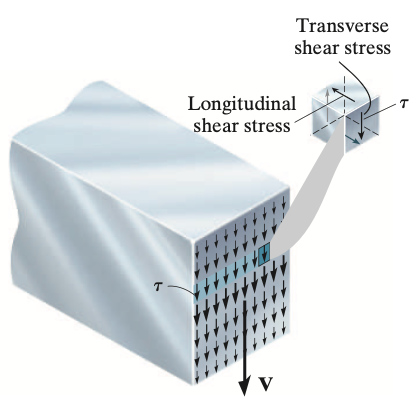
\includegraphics[width=0.4\linewidth]{./figures/f21_1.png}
  \caption{Transverse and longitudinal shear stress.}
  \label{fig:f21_1}
\end{figure}

To illustrate this, we consider the beam made of the three boards shown on \Cref{fig:f21_2}a.
If the top and bottom surfaces of each board are smooth and the boards are not bonded together, then the application of the load $\Vec{P}$ will cause the boards to slide relative to each other.
If the boards instead are bonded together, then the longitudinal shear stress acting in the bonding between the boards will prevent their relative sliding as shown on \Cref{fig:f21_2}b.

\begin{figure} [ht]
  \centering
  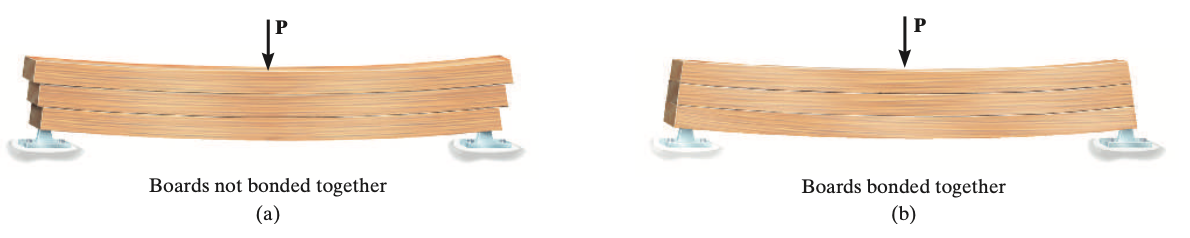
\includegraphics[width=\linewidth]{./figures/f21_2.png}
  \caption{Effect of longitudinal shear stress.}
  \label{fig:f21_2}
\end{figure}

As a result of the shear stress, shear strains will be induced that will tend to distort the cross section in a rather complex manner.


\subsection{The Shear Formula}
As the strain distribution for shear is not easily defined, as in the case of axial load, torsion, or bending, we will have to obtain the shear-stress distribution in an indirect manner.
We will first consider the horisontal force equilibrium of a portion of an element with length $\mathrm{d}x$ taken from the beam as shown on \Cref{fig:f21_3}a.

\begin{figure} [ht]
  \centering
  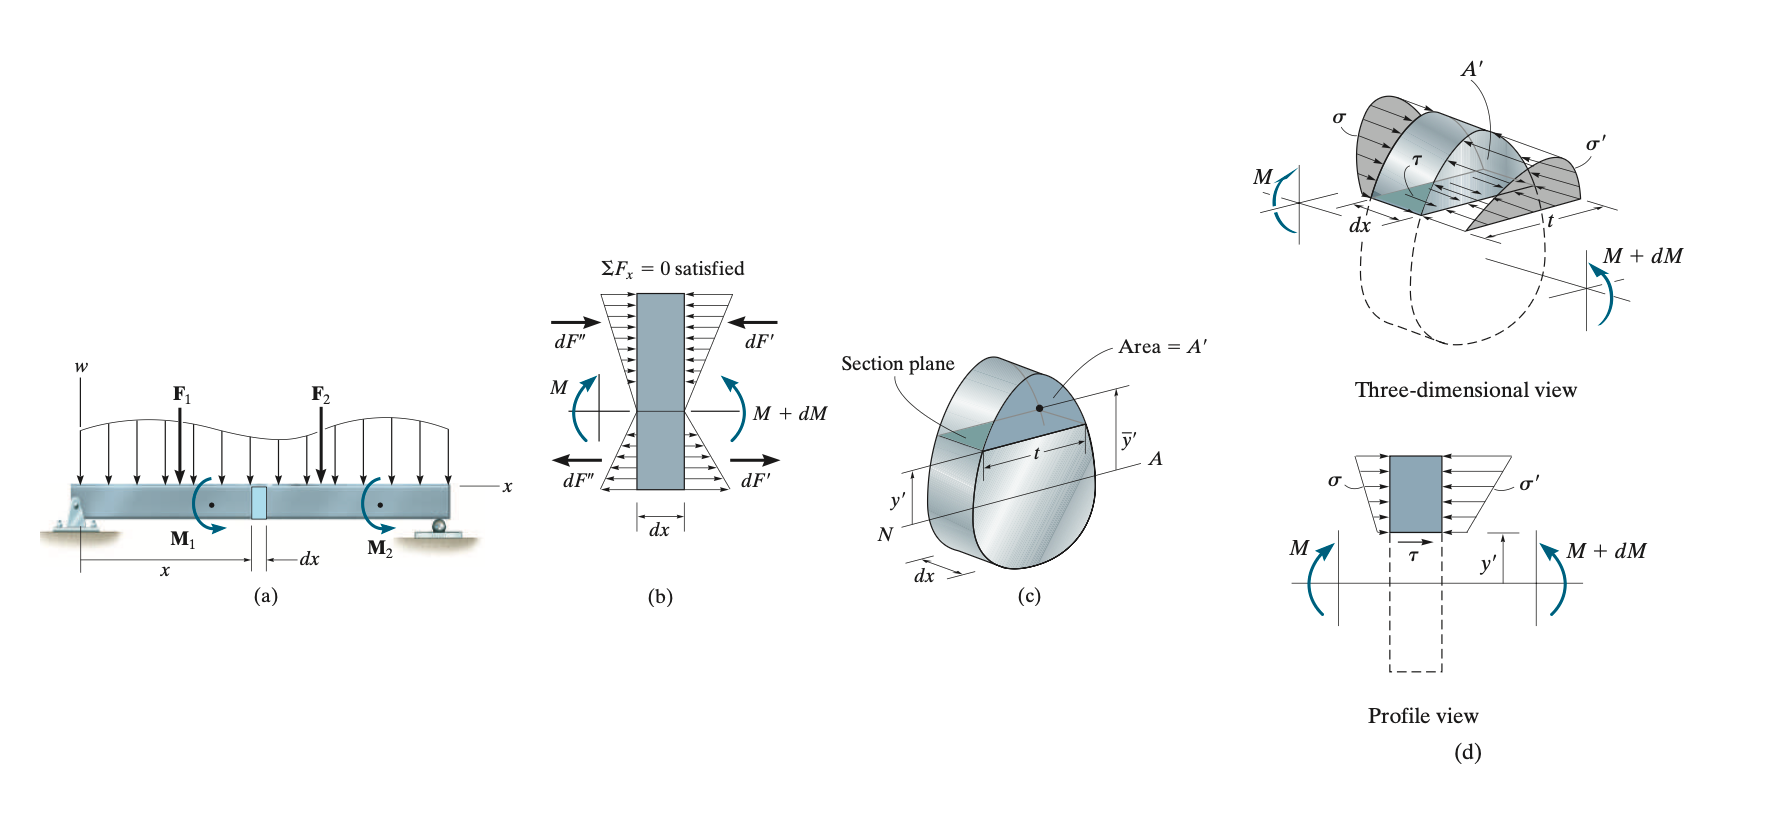
\includegraphics[width=\linewidth]{./figures/f21_3.png}
  \caption{Infinitesimal element of the beam.}
  \label{fig:f21_3}
\end{figure}

A free body diagram of this element is depicted on \Cref{fig:f21_3}b.
The normal shear stress distribution acting on it is caused by the bending moments $M$ and $M + \mathrm{d}M$.
We have excluded the effects of $V$, $V + \mathrm{d}V$ and $w(x)$ since these loadings are all vertical and will therefore not have a horizontal force component.
Here $\sum F_x = 0$ is automatically satisfied since the stress distribution on each side of the element forms only a couple moment and therefore no force resultant is induced.

We now consider the top portion of the element sectioned at $y'$ from the neutral axis, depicted on \Cref{fig:f21_3}c.
It is on this bottom sectioned plane that we want to find the horizontal shear stress.
The top segment has width $t$ at the section, and the two cross-sectional sides each have an area $A'$.
The segment's free body diagram is shown on \Cref{fig:f21_3}d.
As the resultant moment on each side of the element differ by $\mathrm{d}M$, the condition $\sum F_x = 0$ is not satisfied unless a longitudinal shear stress $\tau$ acts over the bottom sectioned plane.
To simplify the analysis, we assume that the shear stress is constant across the width $t$ of the bottom plane.
To find the horizontal force created by the bonding moments, we will assume that the effect of warping due to shear is small, so that it can be neglected.
This assumption is particularly true for the common case os a slender beam.

Using the flexure formula we have:
\begin{align} \label{eq:flexshear}
  - \int_{A'} \sigma' \, \mathrm{d}A' + \int_{A'} \sigma \, \mathrm{d}A' + \tau(t \, \mathrm{d}x) &= 0 \nonumber \\
  - \int_{A'} \left( \frac{M + \mathrm{d}M}{I} \right)y \, \mathrm{d}A' + \int_{A'} \left( \frac{M}{I} \right) y \, \mathrm{d}A' + \tau (t \, \mathrm{d}x) &= 0 \nonumber \\
  \left( \frac{\mathrm{d}M}{I} \right)\int_{A'} y \, \mathrm{d}A' &= \tau (t \, \mathrm{d}x)
.\end{align}
Solving for $\tau$, we obtain
\begin{equation*}
  \tau = \frac{1}{I t} \frac{\mathrm{d}M}{\mathrm{d}x} \int_{A'} y \, \mathrm{d}A'
.\end{equation*}
Here $V = \mathrm{d}M / \mathrm{d}x$.
Also, the integral represents the moment of the area $A'$ about the neutral axis, which we will denote by the symbol $Q$.
Since the location of the centroid area of $A'$ is determined from $\overline{y}' = \int_{A'} y \, \mathrm{d}A' / A'$, we can write the above as:
\begin{equation}
  Q = \int_{A'} y \, \mathrm{d}A' = \overline{y}' A'
.\end{equation}

\begin{figure} [ht]
  \centering
  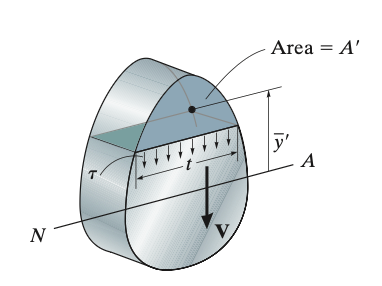
\includegraphics[width=0.5\linewidth]{./figures/f21_4.png}
  \caption{}
  \label{fig:f21_4}
\end{figure}

Substituting, we get the so-called shear formula:
\begin{equation} \label{eq:shearform}
  \tau = \frac{VQ}{I t}
.\end{equation}
With reference to \Cref{fig:f21_4}, $\tau$ is the shear stress in the member located at $y'$ from the neutral axis, $V$ is the shear force, $I$ is the moment of inertia of the entire cross-sectional area calculated about the neutral axis, $t$ is the width of the member's cross section, meassured at $y'$, and $Q = \overline{y}' A'$, where $A'$ is the area of the top portion of the members cross section at plane $y'$ where $t$ is measured, and $\overline{y}'$ is the distance from the neutral axis to the centroid of $A'$.

\paragraph{Calculating Q}
Of all the variables in the shear formula, \Cref{eq:shearform}, $Q$ is usually the most difficult to define.
This represents the \textit{moment about the neutral axis of the cross-sectional area that is above or below the level where the shear stress is to be determined}.
Is is this area $A'$ that is ``held onto'' the rest of the beam by the longitudinal shear stress as the beam undergoes bending, \Cref{fig:f21_3}d.


\subsection{Shear Flow in Built-up Members}
Occasionally in engineering practice, beams are constructed from several composite parts in order to achieve a greater resistance to loading.
When the loads cause the members to bend, a fastener is needed to keep the members from sliding against each other as shown on \Cref{fig:f21_2}.
In order to design these, it is necessary to know the shear force they must resist.
This loading, when measured as a force per unit length of the beam is referred to as a shear flow $q$.

The magnitude of the shear flow is obtained using a procedure similar to the one used for finding the shear stress in the beam.
Doing this one obtains the shear flow formula:
\begin{equation*}
  q = \frac{VQ}{I}
\end{equation*}
where, $q$ is the shear flow, $V$ is the shear force, $I$ is the moment of inertia of the entire cross-sectional area about the neutral axis and $Q = \overline{y}' A'$ where $A'$ is the cross sectional area that is connected to the beam at the juncture where the shear flow is calculated and $\overline{y}'$ is the distance from the neutral axis to the centroid $A'$.

\paragraph{Fastener Spacing}
When segments of a beam are connected by fasteners, such as nails of bolts, their spacing $s$ along the beam can easily be determined,
For example, consider a fastener that can support a maximum shear force of $F$ before it fails.
If these nails are used to construct a simple beam by combining two boards, then the nails must resist the shear flow $q$, between the boards.
The nail spacing is therefore:
\begin{equation*}
  F = q \cdot s
.\end{equation*}

